%% author Martin Monperrus

\section{Introduction}

% PLearn is above all a C++ Library for research in the field of Machine
% Learning. But it also comes with a set of tools and programs, that allow
% you to easily carry out experiments.

PLearn is an open source software for machine learning, with numerous features.
It can be used as an runnable software or as a library. This tutorial will help 
you to discover what is PLearn and how to use it.
I assume that:
\begin{itemize}
\item you have basic concepts in machine learning.
\item you have basic concept in object programming.
\item you have a PLearn binary that runs.
\end{itemize}

\section{A basic classification problem}

\subsection{First steps}
We consider the following classification problem. In a 2-D space, we have two 
classes. The problem is represented on figure \ref{classpb}. 

\begin{figure}
  \center{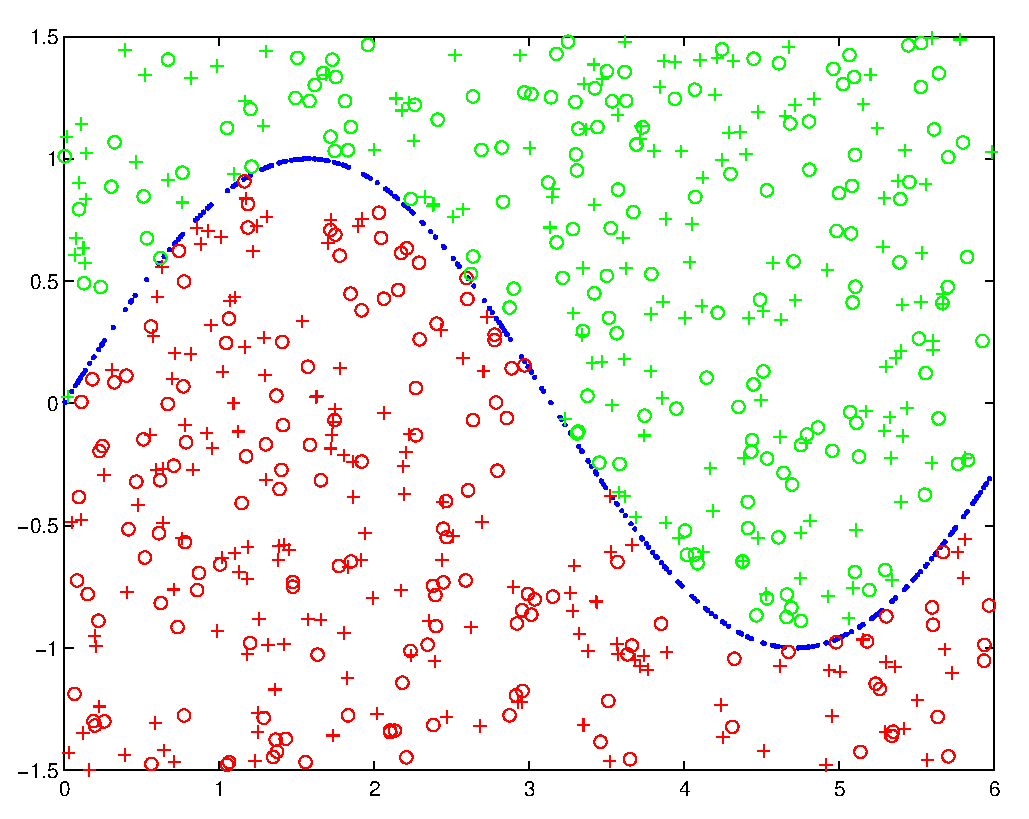
\includegraphics[width=100mm]{class}}
  \caption{In red, the first class. In green, the second one. In blue, the 
analytic decision boundary. The train examples are 0, the test ones +}  
\label{classpb}
\end{figure}

The data are generated with a Matlab script, called 
task1.m\footnote{provided in \texttt{Plearn/examples}, as all the other sources for this tutorial}.The 
script generates boundary.amat, train.amat, test.amat, and space.amat.
% \verbatiminput{../examples/task1.m}

Now, let's train a neural network on this task with PLearn.

We create the PLearn script, a kind of configuration file:
\verbatiminput{../examples/NNet.plearn}

We call this file \texttt{NNnet.plearn}.

Now we have to specify the dataset. In a classification problem, the dataset is 
a set of examples and their associated classes. We have already created such a 
file in Matlab, called train.amat.
Now we have to specify to PLearn that the two first columns of ``train.amat'' 
contain the data, and the last column the class label, which is in ${-1,1}$, 
corresponding to the output of a tanh.

All this tasks are made with the following file, called \texttt{train.vmat}:
\verbatiminput{../examples/train.vmat}

Now, let's train the network with the folllowing command:

\texttt{plearn learner train NNet.plearn train.vmat final.psave}

Then test on the original space:

\texttt{plearn learner compute\_outputs final.psave space.amat 
out.pmat}

We need two additionnals commands to view the result of the network with matlab:

\texttt{plearn vmat convert out.pmat out.amat} converts from a binary to an ascci file.

\texttt{tail +3 out.amat > result.mat} removes meta-information at the beginning of the file.

Then we execute the result\_task1.m script in Matlab to plot the result, as in figure 
\ref{df}.\begin{figure}
  \center{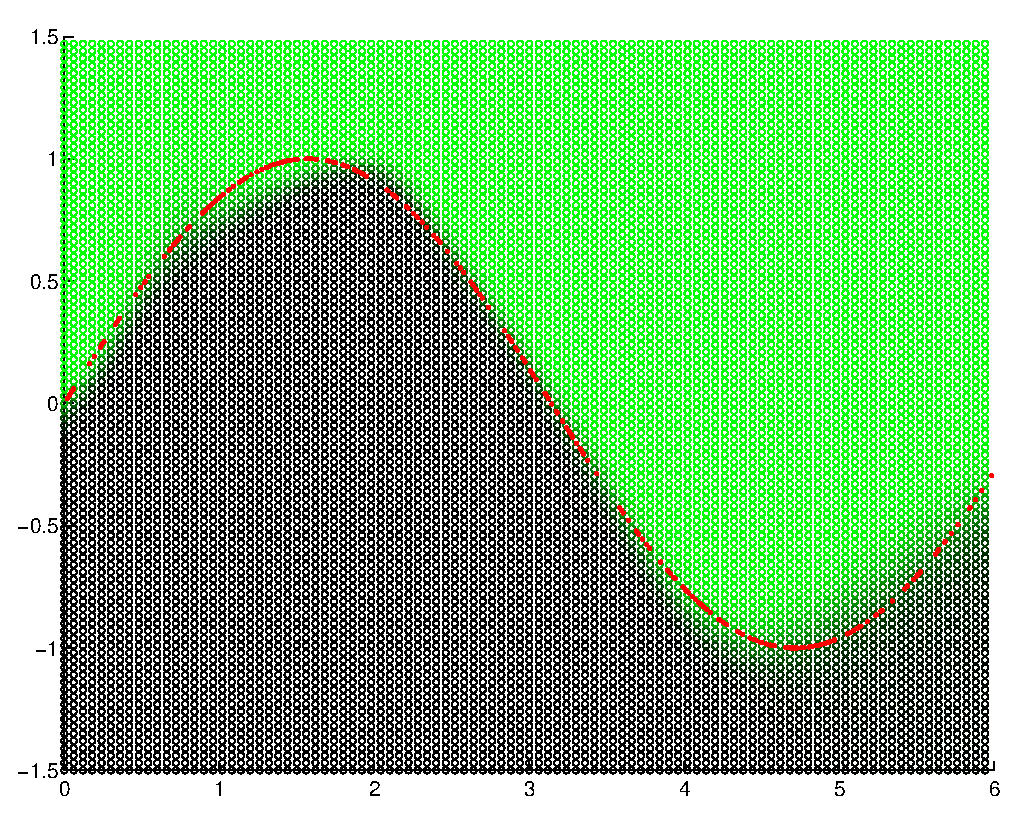
\includegraphics[width=100mm]{decbound}}
  \caption{Analytic and learned boundary}  
\label{df}
\end{figure}

\subsection{What have we done?}

NNet.plearn contains informations about the neural net. train.vmat contains informations about the the dataset.

PLearn is built with a direct help system. For example:

\texttt{plearn help NNet}

\texttt{plearn help AutoVMatrix}

\texttt{plearn help GradientOptimizer}

This commands gives you an accurate information.

Here are the more important thing about PLearn.

\begin{bf}PLearn is an object oriented software. The scripting language is object 
oriented. ``plearn help NameOfTheClass'' gives you the corresponding information
\end{bf}

Note that a lot of others parameters exist for each classes but they have default values.

\section{A second example}

We now consider a regression problem. We want to train a neural network to predict a sinus.

First, we generate the data with the task2.m matlab file.

Then we perform the task within only one script, the following \texttt{regression.plearn}.

\verbatiminput{../examples/regression.plearn}

Let's run Plearn on this script:
\texttt{plearn regression.plearn}

Then test on the original space:
\texttt{plearn learner compute\_outputs tutorial\_task2/Split0/final\_learner.psave space2.amat out.pmat}

We need two additionnals commands to view the result of the network with matlab:

\texttt{plearn vmat convert out.pmat out.amat}

\texttt{tail +3 out.amat > result.mat}

Let's view the result with a matlab script, result\_task2.m:

\begin{figure}
  \center{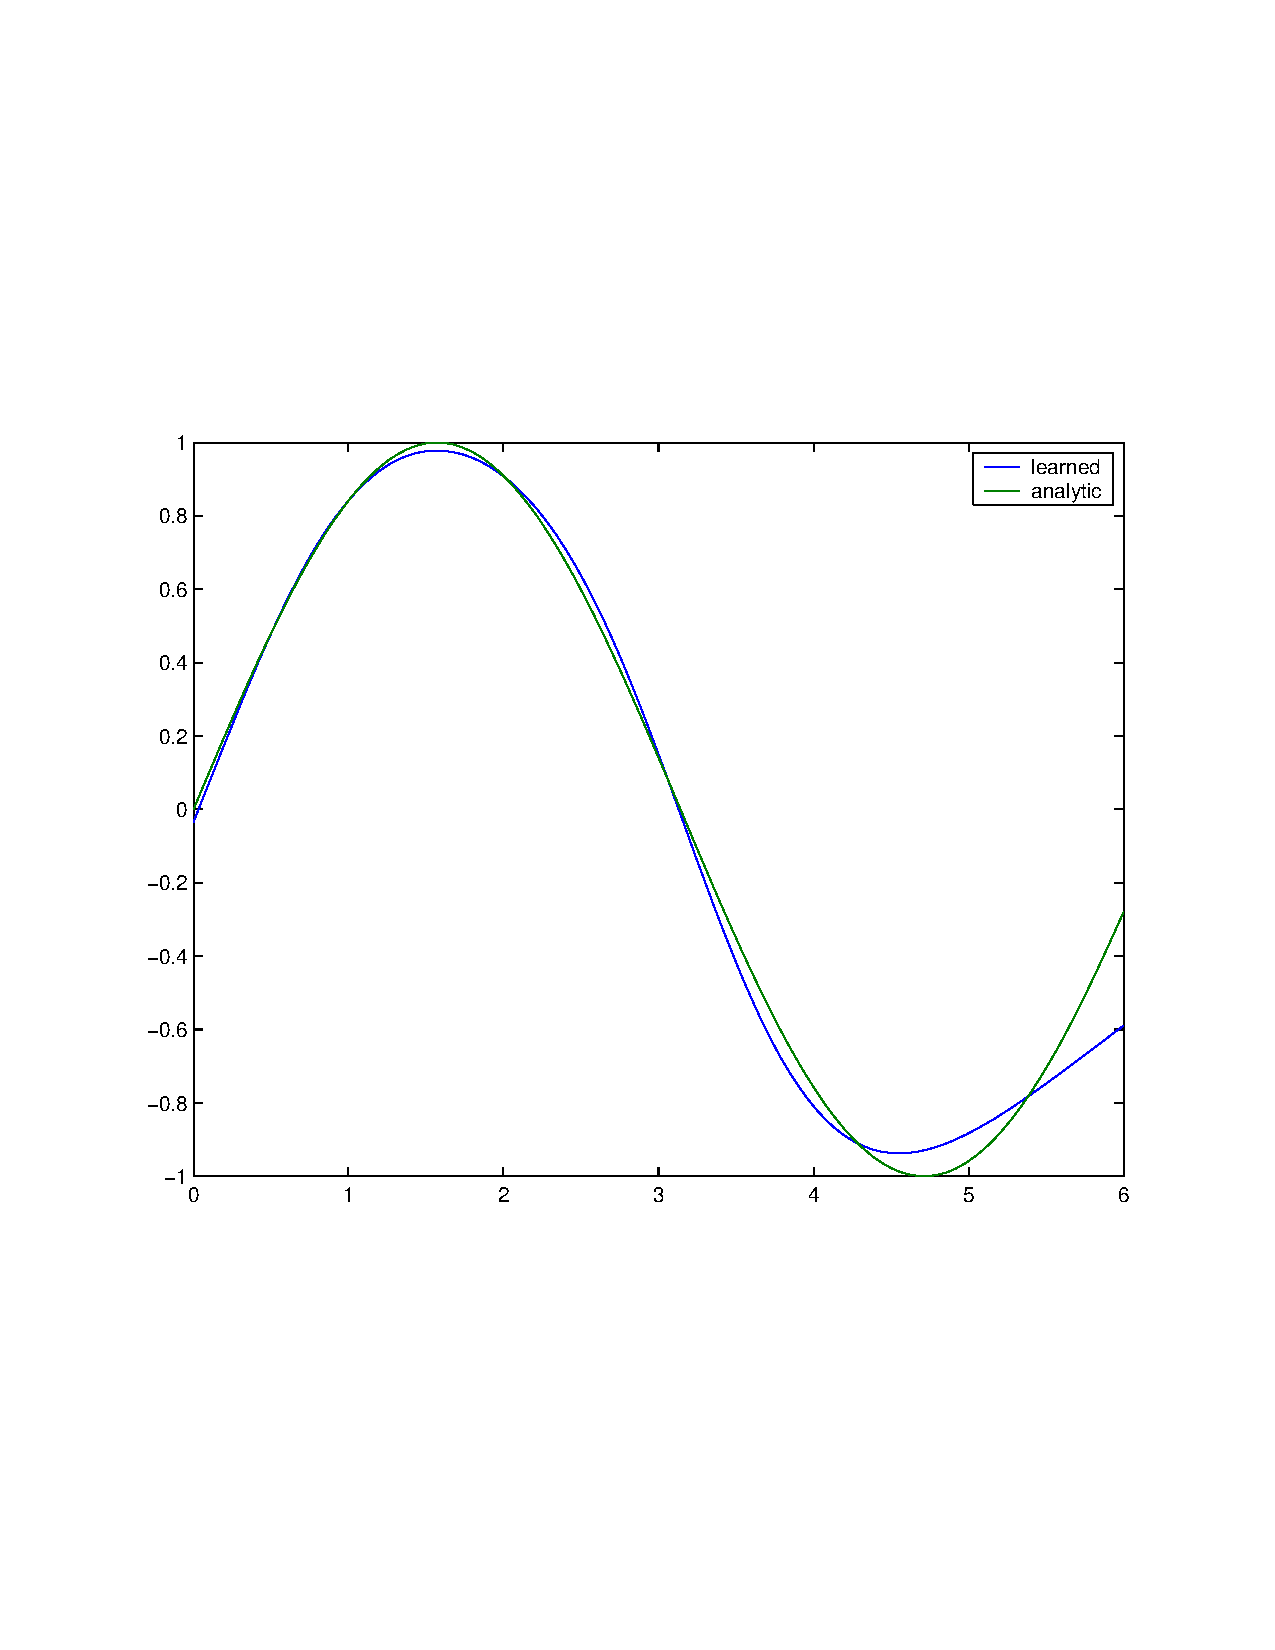
\includegraphics[width=100mm]{reg}}
  \caption{Analytic and learned function}  
\label{reg}
\end{figure}

\subsection{What have we done?}

We encapsulated the experiment in a powerful scriptable class called ``PTester''.

The command \texttt{plearn help PTester} gives you the corresponding information.
Note that a lot of others parameters exist for PTester but they have default values.

Furthermore, explore all the files that a PTester creates:

\begin{verbatim}
cd tutorial_task2/
ls
plearn vmat view split_stats.pmat
plearn vmat view global_stats.pmat
cd Split0
ls
less test1_stats.psave
less final_learner.psave
\end{verbatim}


\section{Conclusion}
This short tutorial shows a small part of PLearn. Continue by yourself and have a nice Plearn time! 



